\section{Results}
\label{section:experiments}

The encoder-decoder network was implemented using PyTorch~\cite{paszke2017automatic} (version \texttt{1.0.1}) and training took place on a single GPU (NVIDIA GeForce GTX 1080 Ti or GTX TITAN X).
For all our experiments we used the KITTI data set~\cite{Geiger2013IJRR} with a total number of 30159 images from which 29000 were used during training and 1159 for validation. Additionally, the KITTI Stereo 2015 dataset~\cite{Menze2015CVPR} provided 200 ground truth disparities which were used for numerical comparisons between models. This evaluation was performed by converting both, the predicted disparities, as well as the sparse ground truth disparities into depth space and capping depth to 80 meters.

We used metrics for numerical evaluation found in Eigen \etal~\cite{eigen2014depth} and present the absolute relative error for our experiments. A table with all metrics for all experiments can be found in Supplement \ref{appendix:full-results}. Additionally, to bring the results of the following sections into perspective, we repeated the baseline implementation 12 times with different random seeds and measured the mean and standard deviation of the error metrics. For the abs. rel. error e.g., we observed a mean of $0.1125$ and a standard deviation of $8.581 \times 10^{-4}$. We also noticed about 25\% of the runs were not able to learn, with the loss staying constant at the initial value. Thus the networks performance was not robust to weight initialization.

Most of the training parameters were adopted from Godard \etal, including the number of epochs, learning-rate, optimization procedure, and data augmentation.
Specifically we trained our network for 50 epochs using the Adam optimizer~\cite{kingma2014adam} ($\beta_1 = 0.9, \beta_2 = 0.999$ and $\epsilon = 10^{-8} $). The initial learning rate of $\lambda = 10^{-4}$ was adjusted according to the batch size (i.e. doubling the learning rate when doubling the batch size).
Separate experiments confirmed that batch size did not affect training results significantly when also doubling the learning rate, hence we decided to use a batch size of 16 and thus $\lambda = 2*10^{-4}$ for our initial learning rate. This learning rate stayed constant for the first 30 epochs of training and was then halved every 10 epochs for the rest of the training. The training duration was 20 hours on average and mostly depended on the GPU and the output stride.
Values for the loss weight hyperparameters $\alpha$ from Section~\ref{sec:methods:depth-estimation} were inherited from the original paper. For these, no further hyperparameter optimizations have been conducted.

For training, the KITTI images were resized from $1275\times375$ to $512\times256$ and the same data augmentation as in the original paper was performed. This included flipping both images horizontally at $50\%$ chance level, as well as uniformly distributed gamma [0.8,1.2], brightness [0.5,2.0] and color shifts [0.8,1.2]. 

% TODO: cityscapes pretraining
For our final selection of models, we also employed cityscapes~\cite{Cordts2016Cityscapes} pretraining, followed by fine-tuning on KITTI. Here we used the same learning-rate and epoch count for both pretraining and fine-tuning.

\subsection{Baseline: Implementation Issues}
\label{sec:experiments:baseline}
Before running experiments with architectural changes, we replicated the original publication's~\cite{Godard_2017_CVPR} results. During this process, we encountered some difficulties:
\begin{figure}[t]
    \centering
    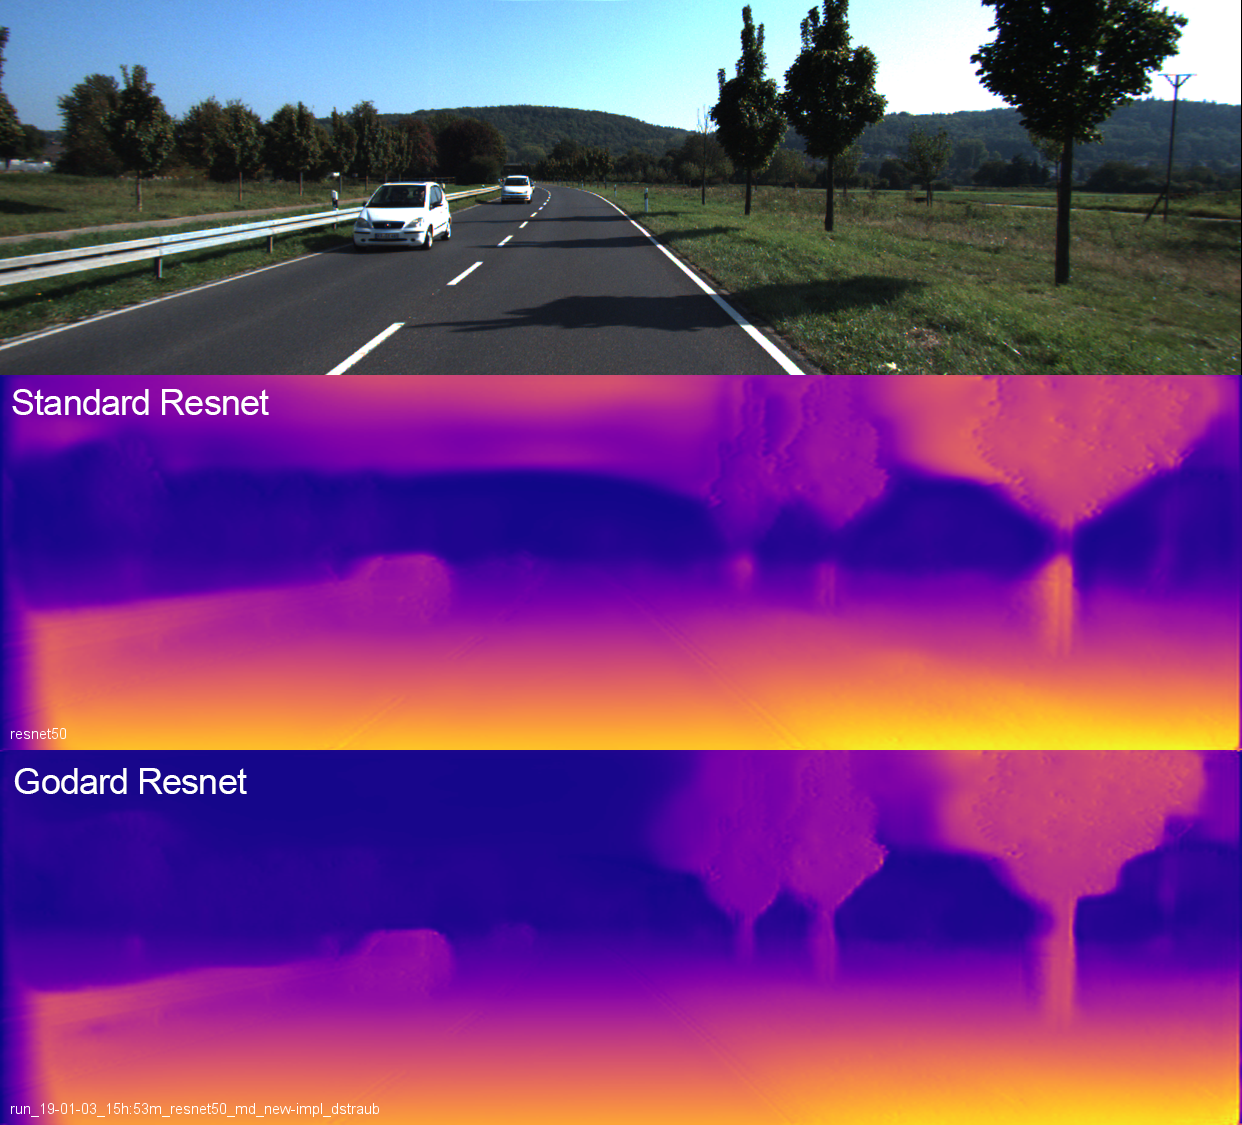
\includegraphics[width=0.8\linewidth]{images/disparities/implementationcomparison_001.png}
    \caption{Comparison between a standard ResNet50 and Godard \etal's ResNet50. Disparities from a standard ResNet50 show severe artifacts in the uniform sky regions, while the modified ResNet50 does not exhibit these problems.}
    \label{fig:sky_artifacts}
\end{figure}
Using the standard ResNet50 architecture from the PyTorch package as the encoder resulted in vastly underestimated depth in the uniform sky regions of the KITTI dataset (see \figurename~\ref{fig:sky_artifacts}, middle row).
This was not present in the disparity maps provided by the original authors~\cite{Godard_2017_CVPR}, which prompted us to investigate Godard \etal's ResNet50 implementation more thoroughly.
We found the following three differences between their implementation compared to a standard ResNet50: 
1) Lack of batch normalization,
2) using nearest neighbor instead of linear upsampling in the decoder and 
3) switching the order of convolutions with \textit{stride} $=1$ and \textit{stride} $= 2$ inside a ResNet block. 
While these differences were tested in isolation, we could not figure out which caused the different behavior of the networks.
However, porting the original TensorFlow implementation line by line to PyTorch fixed the erroneous estimations in homogeneous regions, such as the sky (see \figurename~\ref{fig:sky_artifacts}, bottom row).
Therefore, we used the modified ResNet50 implementation in all following experiments.

\subsection{Output Stride}
\label{section:experiments:output-stride}

\begin{table}

\begin{tabular}{rrrrr}
\toprule
Stride &  Abs. Rel. & Runtime {\tiny $\left(\frac{Min.}{Epoch}\right)$} & Memory (GB) & Param. (M) \\
\midrule
64 &    0.1120 & \textbf{15}  &     \textbf{6.12} &  58.4 \\
32 &    0.1048 &  29  &     8.87 &  58.4 \\
16 &    \textbf{0.1041} &  29  &     8.88 &  58.4 \\
8 &     0.1068 &  43  &    10.61 &  58.4 \\
\bottomrule
\end{tabular}

\caption{Baseline model~\cite{Godard_2017_CVPR} with different output strides (64 being the default): the absolute relative error is optimal at an output stride of 16, while the runtime and memory consumption monotonically increase when decreasing the output stride.}
\label{table:outstride}
\end{table}
Since atrous convolutions can only be effective for images of a certain resolution, which allows the whole kernel to be inside the image, we needed to decrease the output stride of the network (i.e. increase the input size to the ASPP). We conducted an experiment with varying output strides in the baseline model in order to isolate the output stride effect, such that the effect of the ASPP is really due to the ASPP and not merely due to the decreased output stride.
We tested four different output strides (namely 8, 16, 32 and 64) for their effect on predictions and computation time required per epoch.
The results in \tablename~\ref{table:outstride} show that increasing the output stride up to 16 decreases the abs. rel. error on the evaluation, while increasing the training time required for one epoch.
The abs. rel. error increased for output stride 8, among a substantially longer training time.
Unless otherwise specified, we focused on output stride 32 for the following experiments, as this provided the best trade-off between prediction performance and computation time. 

\subsection{ASPP Rates}
\label{section:aspp-rates}
\begin{figure}[t]
    \begin{center}
       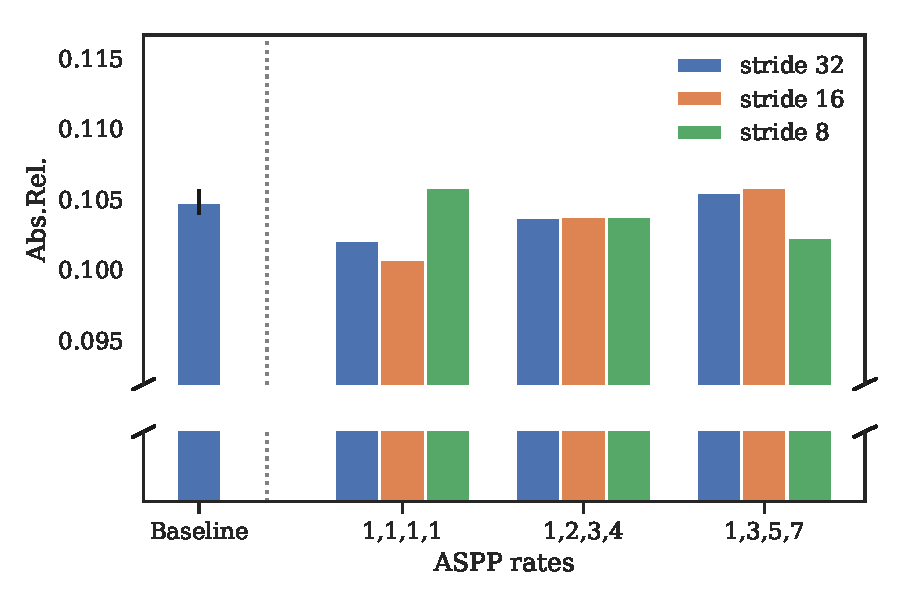
\includegraphics[width=1.0\linewidth]{images/figures/experiment1_AbsRel_os8.pdf}
    \end{center}
   \caption{Absolute relative error of architectures with different ASPP rates. A rate setup of [1,2,3,4] stands for four ASPP modules with an ASPP rate of 1, 2, 3 and 4 respectively.}
\label{fig:aspp-rates}
\end{figure}

In this set of experiments we tested the impact of atrous convolutions with varying atrous rates on the predictive performance of the network. We ran a total of three configurations with atrous rates up to 7 on networks with both output stride 16 and 32 and compared this to the baseline model described in Section~\ref{sec:methods:depth-estimation}.
\figurename~\ref{fig:aspp-rates} shows the abs. rel. error for the different configurations. 

The results suggest that the use of atrous convolutions in the described setup harms the depth estimation performance as seen by the increase in the error. Visual comparison of reconstruction error maps (see supplementary \ref{appendix:reconstruction-error}) also show no apparent differences between the different atrous rates. The model which uses four standard convolutions (\textit{rate = 1}) performed best against models with an increasing atrous rate, and is even slightly superior to the baseline.
For an output stride of 8, the effect's direction is inverted, which suggests that atrous convolutions might help on larger images. This was not investigated further, since models with output stride 8 took significantly longer to train and both output stride 16 and 32 outperform the output stride 8 model. 

\subsection{Number of ASPP Modules}
\label{section:experiments:num-aspp-modules}
% Number of ASPP modules figure
\begin{figure}[t]
    \begin{center}
       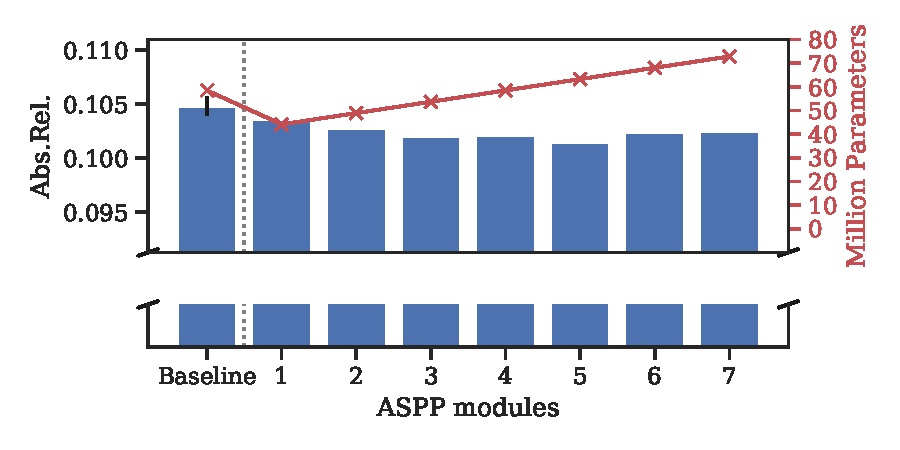
\includegraphics[width=1.0\linewidth]{images/figures/experiment2_AbsRel.pdf}
    \end{center}
   \caption{Absolute relative error of architectures with a different number of ASPP modules. The error bar indicates the standard deviation of the abs. rel. error of our baseline implementation. Additionally, the number of network parameters is plotted for each architecture.}
\label{fig:long}
\end{figure}
Since the network with four standard convolutions in parallel inside the ASPP performed best, we investigated the impact of the number of these convolutional layers.
\figurename~\ref{fig:long} shows the abs. rel. error for models with increasing number of standard convolutions in the ASPP, along with the number of parameters.
One can see, that adding one convolutional layer increases the parameter count by about 4 million, while slightly improving error metrics on the evaluation. This trend starts to decline after more than 5 convolutions are added. 

\subsection{Atrous Convolutions in the Encoder}\label{section:experiments:atrous-encoder}
In the previous, we saw that adding an ASPP module at the end of the encoder, which was successfully done in the DeepLab Architecture for segmantic segmentation~\cite{chen2018deeplab, chen2018encoder}, impaired depth estimation when atrous rates larger than 1 were used.
Therefore, we asked whether depth prediction would benefit from employing atrous convolutions with different rates between or within earlier layers of the encoder (see supplementary \figurename~\ref{fig:appendix:aspp-encoder} and \figurename~\ref{fig:appendix:resnet-atrous}). 

In the first experiment we placed the entire ASPP module between ResNet block 1 and 2 to obtain feature responses at different spatial scales at an earlier stage of the encoder.
At this stage the image has only been resized to $64\times32$ corresponding to an output stride of 8. As an initial exploration, we compared a model with only standard convolutions  (rates [1,1,1,1]) against a model with atrous rates [1,6,12,18] (the default values in DeepLab~\cite{chen2018deeplab}). The model with only standard convolutions performed better than the one with atrous convolutions (see supplementary Table~\ref{table:appendix:aspp-encoder}). Thus, we did not further explore this direction and focused on placing the ASPP after the encoder.

In the second experiment we employed atrous convolutions within the ResNet blocks themselves. Again, all other ASPP rates larger than 1 harmed the depth prediction performance as can be seen by an increase in the error metrics compared to the baseline (see supplementary \tablename~\ref{table:appendix:atrous-encoder}).

\subsection{Evaluation on Virtual KITTI}\label{section:vkitti}
Our goal is to evaluate whether atrous convolutions help with monocular depth estimation, especially if they improve the sharpness at object boundaries. Since the KITTI Stereo 2015 ground truth data is rather sparse, it might not contain data points at exactly those most relevant positions at object boundaries. Synthetic data, on the other hand, provides exact ground truth depth at every single pixel. For this reason, we evaluated the models presented in the previous sections on the Virtual KITTI (VKITTI) dataset~\cite{Gaidon:Virtual:CVPR2016}. Because it only provides monocular images, we could not use it for training but only for evaluation. VKITTI contains clones of five sequences from the original KITTI Vision Benchmark Suite~\cite{geiger2012we} in different weather conditions. To keep these weather conditions identical to the training set, we only chose those sequences that are exact clones of the original sequences, yielding 2126 images in total.
\begin{figure}
    \centering
    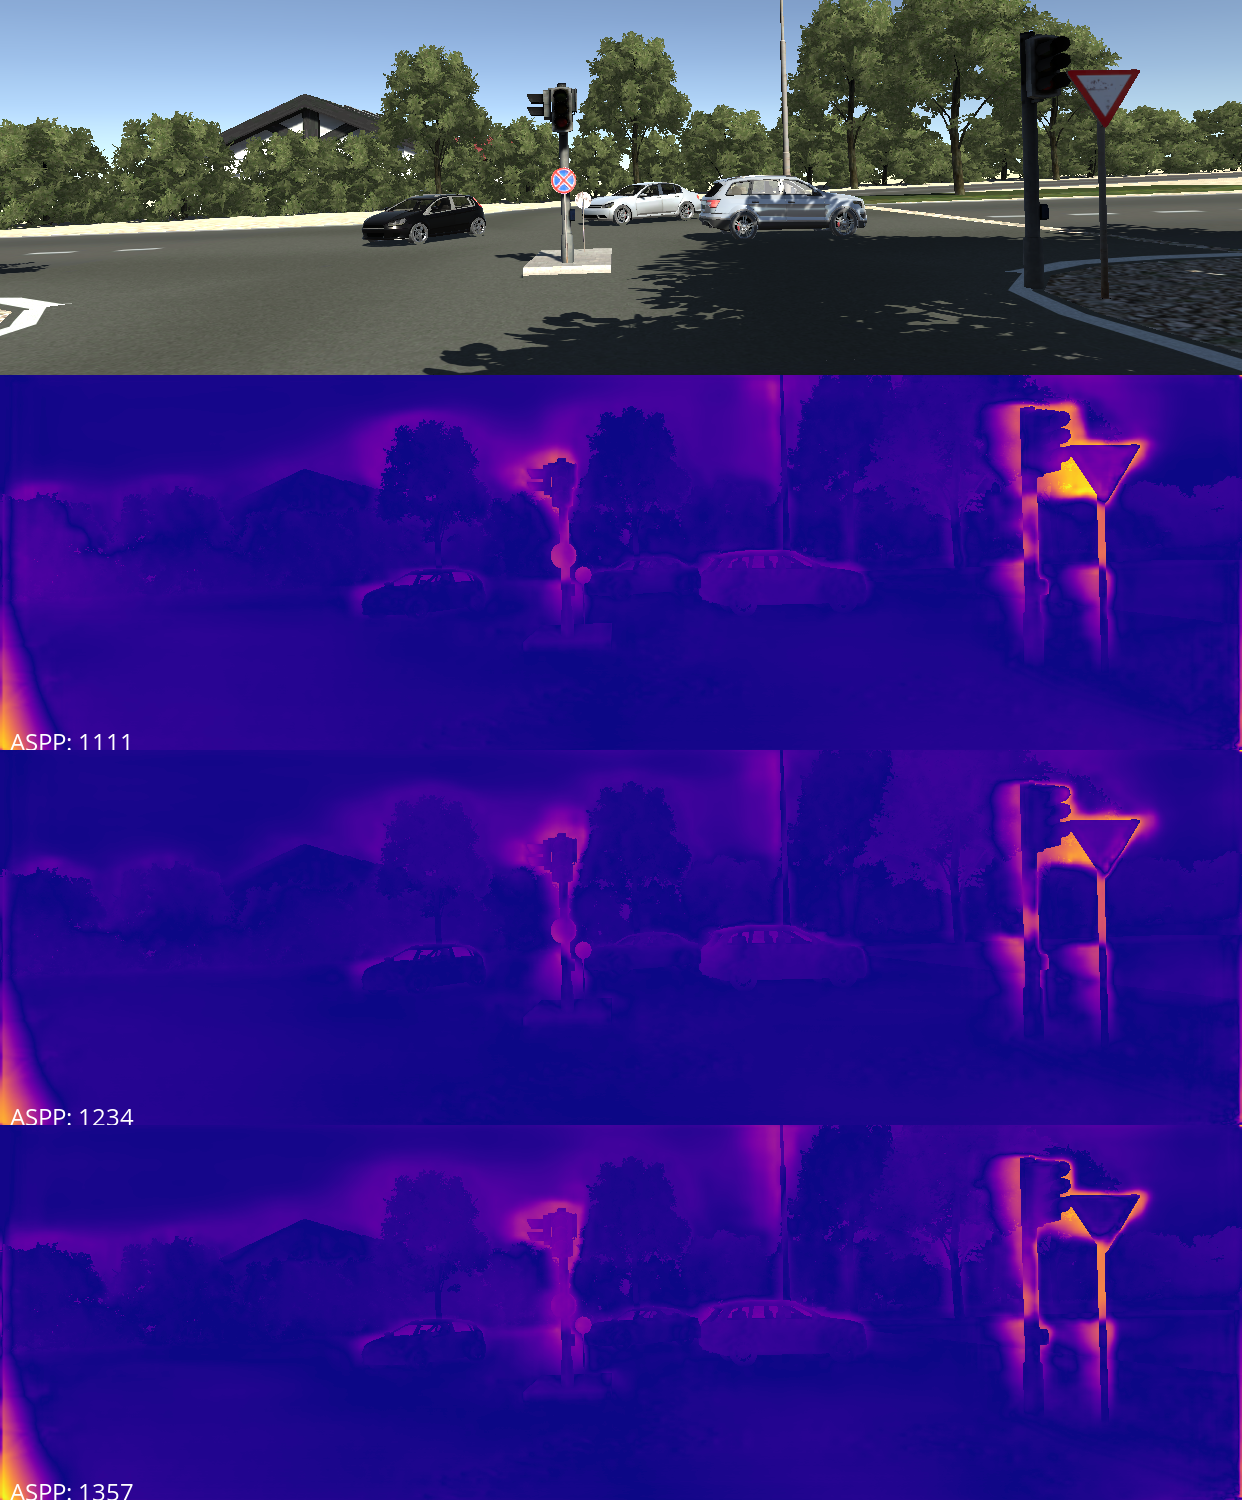
\includegraphics[width=0.85\linewidth]{images/visual_comparisons/aspp-rates-vkitti/concat_383.png}
    \caption{Disparity error maps (absolute difference between predicted and ground truth disparity) on VKITTI. Atrous rates from top to bottom: [1,1,1,1], [1,2,3,4], [1,3,5,7]. Error maps for additional images are available in the supplementary \figurename~\ref{fig:appendix:vkitti}.}
    \label{fig:vkitti}
\end{figure}

% Keep table here due to placement issues
\begin{table*}[h!]
   \centering
   \small
   \setlength{\tabcolsep}{4pt}
   \begin{tabular}{lrllrrrrrrrrr}
\toprule
 Model & Output-stride &     ASPP &  Abs.Rel. &  Sq.Rel. &   RMSE &  Log RMSE &     a1 &     a2 &     a3 &      Params (M) & $\Delta$ Abs. Rel. (\%)\\
\midrule
       Godard & 64  &      - &    0.0970 &   0.8960 &  5.093 &     0.176 &  0.962 &  0.962 &  0.986 &         58.4 & -- \\
       Godard & 16 & - & 0.0955 & 0.8752 &      4.937 &      0.174 &     0.881 &      0.961 &    0.984 & 58.4 & 2.57 \\
            Ours (A) & 16 &  1-1-1-1 &    \textbf{0.0927} &   \textbf{0.8132} &  \textbf{4.865} &     \textbf{0.168} &  \textbf{0.888} &  \textbf{0.967} &  \textbf{0.987} &         58.4 & \textbf{4.43} \\
            Ours (B) & 16 &   1 &    0.0944 &   0.8446 &  5.011 &     0.174 &  0.884 &  0.963 &  0.986 &         \textbf{44.1} & 2.68 \\ \bottomrule \end{tabular}
   \caption{Final model comparison.
   Each model was pretrained on the Cityscapes dataset and evaluated on KITTI Stereo 2015 after applying postprocessing as in \cite{Godard_2017_CVPR}. 
   The last column measures the relative difference of the abs. rel. error to the original model from Godard~\etal~\cite{Godard_2017_CVPR}.}
   \label{table:best-models}
\end{table*}
\figurename~\ref{fig:vkitti} shows disparity error maps for the models with different atrous rates from Section \ref{section:aspp-rates} at output stride 32. As on KITTI, all models have problems predicting disparity accurately at the object boundaries. Upon visual inspection of the disparity maps, there is no apparent difference between the models with different atrous rates. Numerical evaluation did also not provide any clear conclusions w.r.t. the effectiveness of atrous convolutions.

\subsection{Improvement over Baseline}
% Best models table

Summarizing the previous experiments, \tablename~\ref{table:best-models} shows our most interesting models in comparison to the baseline model of Godard \etal~\cite{Godard_2017_CVPR} and illustrates some trade-offs when making architectural decisions.
\begin{figure}
    \centering
    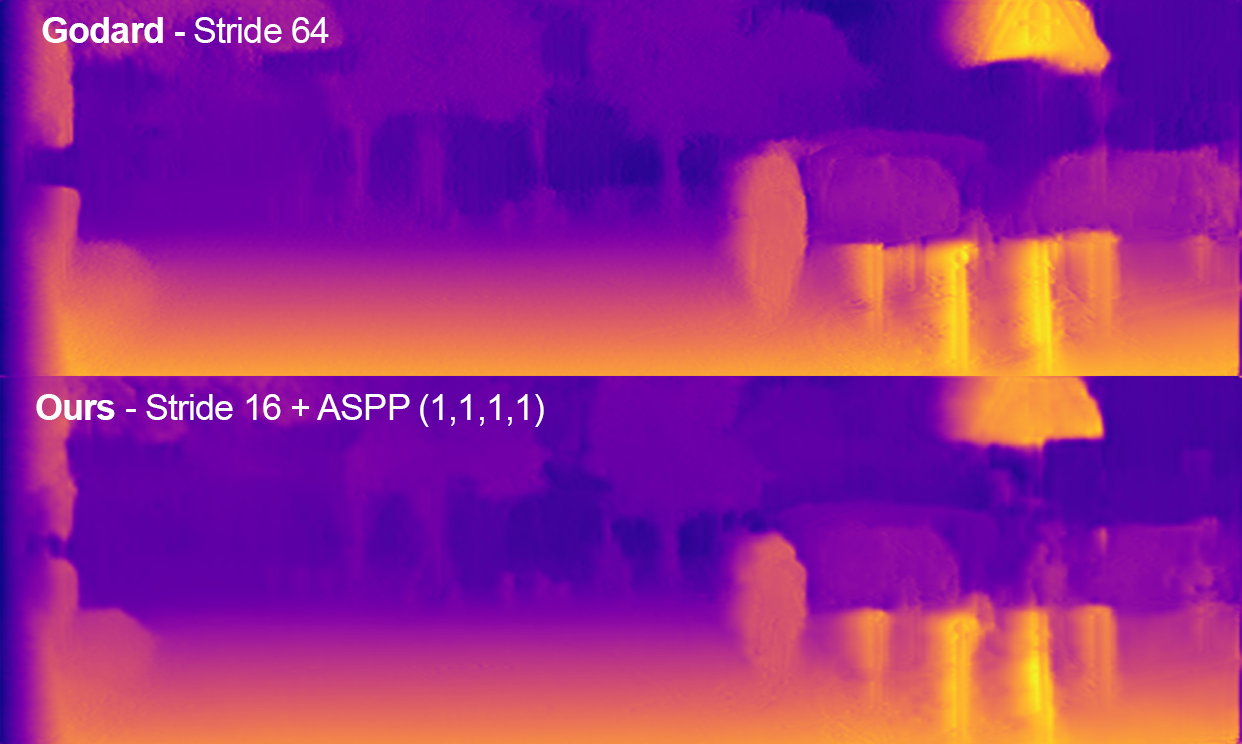
\includegraphics[width=0.8\linewidth]{images/disparities/final_godard_comparison.png}
    \caption{Disparity map comparison of our best model to the baseline~\cite{Godard_2017_CVPR}. There are no obvious visual differences.}
    \label{fig:final-comparison}
\end{figure}
Our best performing model, using an output stride of 16 and four ASPP modules with an atrous rate of 1, achieves an improvement of 4.43\% in the abs. rel. error over the baseline model while having the same number of parameters (model A). There is, however, no clear improvement in terms of visual inspection of the disparity maps (see \figurename~\ref{fig:final-comparison}.
When we further degenerate the ASPP block to only use the very first $1 \times 1$ module, we can reduce the number of parameters by 24.5\%, while still achieving an improvement of 2.68\% over Godard \etal~\cite{Godard_2017_CVPR} (model B).

